%! TeX root = thesis.tex
\chapter{Methodology}\label{methodology}
\IMRADlabel{methods}

\section{Overview}
Would this be better as a numbered list?
The basic premise is to segment the given model into primitive surfaces, such as plane, cylinder, cone, etc.
Each surface is unwrapped and simplified to its 2D representation, which undergoes a 2D segmentation to produce convex regions.
Upon each convex region a local path is planned.
The order in which each region is traversed by the robot is determined via a modified Traveling Salesman Problem (TSP).
The classic TSP creates a closed loop of nodes, but in this application the start and end points of the salesman's path need not be the same.
Finally, the waypoints of the complete path are converted to actuator positions and sent via XMLRPC to the connected robotic arm and rotary table to be executed.
Figure \ref{fig:overview} gives a graphical overview of the procedure's main steps.

\begin{figure}[ht]
	\centering
\begin{tikzpicture}
	\newdimen\dx
	\dx=6mm
	% nodes
	\node[] (Mesh) {Mesh};
	\node[FC-Node] (3DSeg) [right=\dx of Mesh] {3D Segmentation};
	\node[FC-Node] (GeoSimp) [right=\dx of 3DSeg] {Geometry Simplification};
	\node[FC-Node] (2DSeg) [right=\dx of GeoSimp] {2D Segmentation};
	\node[FC-Node,text width=27mm] (Bpath) [below=10mm of Mesh, xshift=10mm] {Cellular path planning};
	\node[FC-Node,text width=30mm] (TSP) [right=\dx of Bpath] {Modified TSP};
	\node[FC-Node,text width=20mm] (InvKin) [right=\dx of TSP] {Inverse Kinematics};
	\node[text width=20mm] (Poses) [right=\dx of InvKin] {Actuator Poses};
	% connections
	\draw [FC-Arrow] (Mesh) -- (3DSeg);
	\draw [FC-Arrow] (3DSeg) -- (GeoSimp);
	\draw [FC-Arrow] (GeoSimp) -- (2DSeg);
	\draw [FC-Arrow, rounded corners=5pt] (2DSeg.south) |-| (Bpath.north);
	\draw [FC-Arrow] (Bpath) -- (TSP);
	\draw [FC-Arrow] (TSP) -- (InvKin);
	\draw [FC-Arrow] (InvKin) -- (Poses);
\end{tikzpicture}
	\caption{Graphical overview of the path planning and execution procedure}
	\label{fig:overview}
\end{figure}

\section{3D Segmentation}
Segmentation in 3D consists of breaking the model into primitive surfaces, which have (easily) solvable mappings from 3D to 2D.
This is done by applying Watershed segmentation to the mesh as a whole and attempting to classify the resultant mesh sections as a certain primitive.
Watershed segmentation is imperfect, and sometimes yields mesh sections comprised of multiple primitive types.
In such cases the composite mesh section undergoes Watershed segmentation again, but with a lower merge threshold (see \ref{ws_seg}), so that it might be split into multiple mesh sections.
This procedure is displayed visually in figure \ref{fig:Seg3D}.

\begin{figure}
	\centering
\begin{tikzpicture}[]
	\newdimen\dx
	\dx=6mm
	% nodes
	\node (Mesh) {Complete Mesh};
	\node[FC-Node, text width=30mm] (WS) [right=\dx of Mesh] {Watershed Segmentation};
	\node[FC-Node, text width=30mm] (PrimCl) [right=\dx of WS] {Primitive Classification};
	\node[text width=25mm, align=center] (MRs) [right=\dx of PrimCl] {Classified Mesh Sections};
	% connections
	\draw [FC-Arrow] (Mesh) -- (WS);
	\draw [FC-Arrow] (WS) -- (PrimCl);
	\draw [FC-Arrow] (PrimCl) -- (MRs);
	% \path (PrimCl.south) -- node[below=5mm of PrimCl] (CompPrim) {Composite Primitive} (WS.south);
	% \draw [FC-Arrow, rounded corners=5pt] (PrimCl.south) |- (CompPrim) -| (WS.south);
	\draw [FC-Arrow, rounded corners=5pt] (PrimCl.south) -- +(0,-0.4) -| (WS.south)
		node[pos=0.5,below right]{Composite primitives};
	% Segmentation 3D container node
	\draw[thick, dashed, rounded corners=8pt] ($(WS.north west)+(-0.3,0.3)$) rectangle ($(PrimCl.south east)+(0.3,-1.2)$);
	\node [] at (5.7, 1.1) {3D Segmentation};
	% TODO: make this diagram more flexible
\end{tikzpicture}
	\caption{Graphic depiction of the 3D segmentation procedure}
	\label{fig:Seg3D}
\end{figure}

\subsection{Watershed Segmentation}\label{ws_seg}
A watershed, according to the North American usage, is an area of land, in which all streams and rainfall drain to a common body of water\cite{USGS_Watersheds}, also commonly called catchment basins.
Somewhat confusingly, the rest of the English speaking world uses ``Watershed'' to refer to the high elevation regions that separate said catchment basins.
Watershed segmentation originally comes from image processing, where it is used for image segmentation\cite{ImageSegWS, DigitalImageProc}.
It works by applying a ``height function'' to the input image and forming image regions divided by ``high'' areas.
A common ``height function'' in image processing is the gradient of the image\cite{ImageSegWS}.
Mangan and Whitaker first applied this concept to 3D meshes, replacing pixels for the mesh's vertices and the image gradient for the mesh curvature\cite{Watershed}.

\subsubsection{Basic Procedure}
Mangan and Whitaker's algorithm consists of 6 steps:
\begin{enumerate}
	\item Apply the height function to each vertex
	\item Find and label each local minima
	\item Find flat areas and classify them as either a minimum or plateau
	\item \label{plateau_step} Loop through the plateaus and allow each to descend to a labeled region
	\item Descend from all remaining vertices to labeled regions
	\item Merge regions whose watershed depth is below a given threshold
\end{enumerate}

Their algorithm was modified throughout this project, as described in the following sections.
Atkar et al's Watershed segmentation implementation also helped inspire the implementation in this work\cite{HierSurfSeg_for_autobody_painting}.
Their graphical depiction of Watershed segmentation is shown below in figure \ref{fig:ws_1570179_steps}.
% In addition to the mesh to be segmented, a merge threshold value is provided to Watershed.
% This threshold value is described in greater detail in \ref{sec:shallow_merge}.
\begin{figure}[htb]
	\centering
	% TODO: recreate this image with tikz
	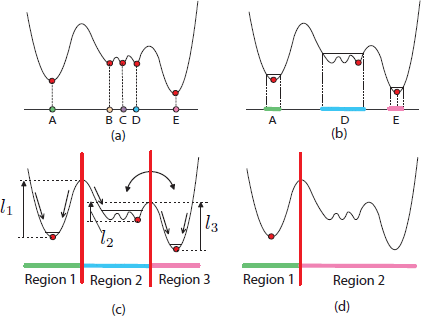
\includegraphics[width=0.5\linewidth]{../resources/watershed/1570179_WS_steps.png}
\caption{
Graphical depiction of Atkar et al.'s Watershed segmentation implementation.\cite{HierSurfSeg_for_autobody_painting}
}
	\label{fig:ws_1570179_steps}
\end{figure}

In figure \ref{fig:ws_1570179_steps} subfigure (a) shows Mangan and Whitaker's step 2: locating and labeling each local minima.
Region 1 in subfigure (c) depicts the original step 5: descent to a minimum, and regions 2 and 3 in the same subfigure show step 6: the merging of shallow regions into deep ones.
The step shown in subfigure (b) is of Atkar et al.'s own design, and due to its adaptation in this work, is described in the section on \textit{minima expansion}.
Figure \ref{fig:ws_1570179_steps} concludes with the end result of Watershed in subfigure (d).

\subsubsection{Region Initialization}
In this work's implementation the curvature values and derivative thereof are calculated once for the whole mesh prior to the first Watershed pass.
Watershed step 0, applying the height function to the mesh, is shown in figure \ref{sfig:ws_dk}.
This work's version of Watershed begins by creating mesh regions from each local minima.
Here, local minima includes local plateaus.
Thus, if a region of the mesh is found whose vertices' curvature are all roughly equal and less than that of their neighbors, it is a minima plateau.

\begin{figure}[htb]
	\centering
	\begin{subfigure}{0.45\textwidth}
		\centering
		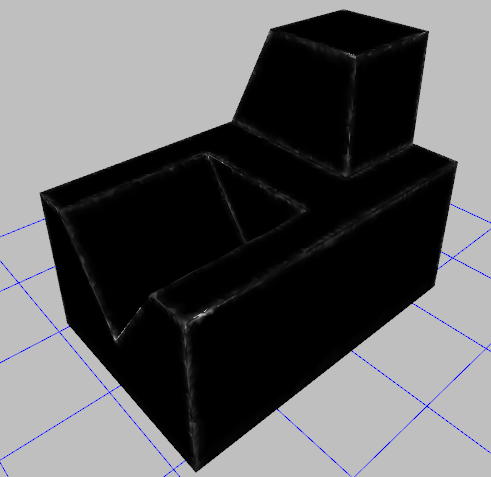
\includegraphics[width=\linewidth]{../resources/watershed/fc028_WS0.png}
		\caption{Watershed step 0: Apply height function to mesh. White indicates high curvature and black indicates low curvature.}
		\label{sfig:ws_dk}
	\end{subfigure}
	\hfill
	\begin{subfigure}{0.45\textwidth}
		\centering
		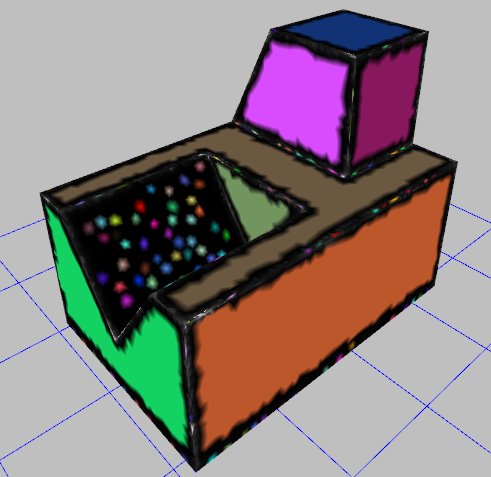
\includegraphics[width=\linewidth]{../resources/watershed/fc028_WS1.png}
		\caption{Watershed step 1: Mesh region initialization. Each color is a separate mesh region.}
		\label{sfig:ws_1}
	\end{subfigure}
\caption{
Watershed segmentation steps 0 and 1 shown applied to test object ``fc028\_e''.
}
\end{figure}

Figure \ref{sfig:ws_1} shows the result of region initialization on the test object ``fc028\_e''.
Because the surfaces of the test object are perfectly flat, the horizontal and vertical surfaces exhibit large plateaus.
The lack of plateaus on the inclined surface is most likely due to floating point errors in the vertex positions on the inclined surface.

\subsubsection{Minima Expansion}
This step was adopted from Atkar et al.'s implementation of Watershed segmentation\cite{HierSurfSeg_for_autobody_painting}.
Each mesh region expands up to a pre-set depth, absorbing any regions encountered.
Although not essential to the segmentation results, it facilitates subsequent steps by effectively filtering high frequency noise and features from the mesh.
It is worth noting that Watershed segmentation overall would work without \textit{minima expansion}, but would be slightly slower because the region merging in steps 4.1 and 4.2 are a little more computationally expensive than region merges during \textit{minima expansion}.

\begin{figure}[htb]
	\centering
	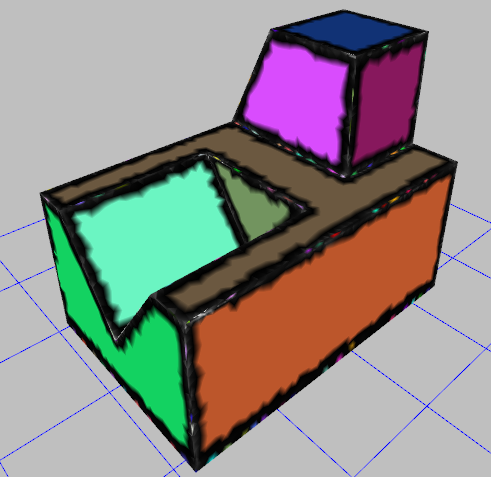
\includegraphics[width=0.5\linewidth]{../resources/watershed/fc028_WS2.png}
\caption{
Test object ``fc028\_e'' post Watershed segmentation step 2.
}
	\label{fig:ws_2}
\end{figure}

Figure \ref{fig:ws_2} shows the result of \textit{minima expansion} on the test object.
Because the variation in height among the vertices of the inclined surface was minimal, one of the initial local minima was able to expand to most of the inclined surface's area.

\subsubsection{Descent to Minima}
From each un-assigned vertex a trail following the path of steepest descent is started.
When a mesh region is encountered, the traversal ends and all path vertices are added to the encountered mesh region.
Plateaus encountered during the descent are added to the traversal path.
In this way, Mangan and Whitaker's step \ref{plateau_step} is effectively split between Region Initialization and Descent to Minima.
A way to visualize this step is by placing an imaginary drop of water at an un-assigned vertex of the object.
All vertices touched by the water droplet as it descends the height map of the object's surface are added to the region that eventually catches the droplet.
Post \textit{descent to minima} all vertices have been assigned to a mesh region and the mesh has been segmented.
Figure \ref{fig:ws_3} shows the result of \textit{descent to minima} on the test object.

\begin{figure}[htb]
	\centering
	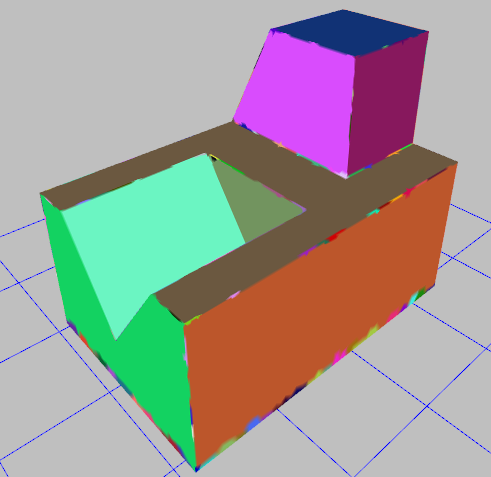
\includegraphics[width=0.5\linewidth]{../resources/watershed/fc028_WS3.png}
\caption{
Test object ``fc028\_e'' post Watershed segmentation step 3: Descent to minima
}
	\label{fig:ws_3}
\end{figure}

\subsubsection{Mini-Merge}
As noted by Mangan and Whitaker, Descent to Minima will segment the given mesh, but in all likelihood it will be overly segmented.
Their solution was to merge shallow regions into adjacent deeper regions (see subsequent section on \textit{shallow merge}).
Through testing small high curvature regions were observed, that due to their high curvature did were not merged into any of the larger more useful regions.
To combat this, the ``Mini-Merge'' step was developed to merge regions deemed too small to be worth keeping.
The merge condition changed throughout development, from a fixed number of vertices threshold, to a threshold relative to the total number of vertices in the mesh undergoing Watershed segmentation, to the condition that the number of perimeter vertices in the region be fewer than 50\% of the region's vertices.
(reword previous sentence?)
The \textit{mini-merge} procedure is shown in algorithm \ref{alg:WS:mini_merge}.

\begin{algorithm}[htb]
\caption{Mini-Merge}\label{alg:WS:mini_merge}
\begin{algorithmic}[1]
\Function{miniMerge}{Mesh sections $S$}
	% \State Sort $S$ by vertex count in ascending order
	\For{$s$ in $S$}
		% \State $s_{small} \leftarrow S$.first
		\If{$s$.small()}
			\State $s_{lowside} \leftarrow s$.findLowSideNeighbor()
			\State $s_{lowside}$.absorb($s$)
			% \State $S$.erase($s$)
		\EndIf
	\EndFor
\EndFunction
\end{algorithmic}
\end{algorithm}

\textit{Mini-merge} iterates through each mesh section, checking each if it meets the aforementioned merge condition.
When a small region is found, the region adjacent its low side is sought, which then absorbs the small region.
% Mesh regions that trigger the merge condition are merged into the mesh region adjacent their shallow side.
The method to find the low-side adjacent neighboring mesh region is shown below in algorithm \ref{alg:MR:low_side_neighbor}.

\begin{algorithm}[htb]
\caption{Find low side neighbor}\label{alg:MR:low_side_neighbor}
\begin{algorithmic}[1]
\Function{findLowSideNeighbor}{}
	\For{$p_{perimeter}$ in $P_{perimeter}$}
		\For{point $p_{adj}$ adjacent to $p_{perimeter}$}
			\If{$p_{adj}$ not in this region AND $p_{adj}$ is in bounds}
				\State \textbf{return} $p_{adj}$.meshRegion
			\EndIf
		\EndFor
	\EndFor
\EndFunction
\end{algorithmic}
\end{algorithm}

The receiving mesh region is found by searching the vertices adjacent to the mini region's lowest perimeter vertex.
If for some reason no valid mesh region adjacent to that vertex is found, the neighborhoods of the remaining perimter vertices are checked in ascending order until a valid mesh region is found.

\begin{figure}[htb]
	\centering
	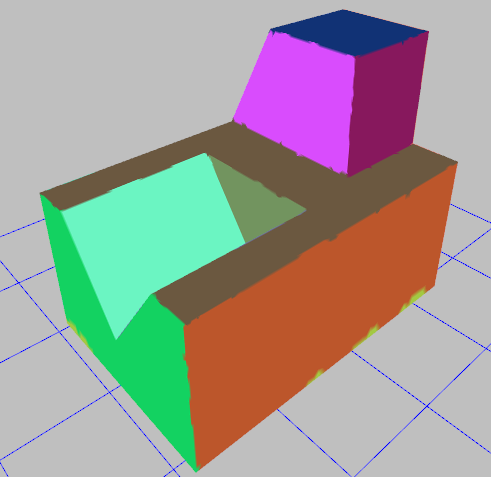
\includegraphics[width=0.5\linewidth]{../resources/watershed/fc028_WS4.1.png}
\caption{
Watershed segmentation step 4.1 shown applied to test object ``fc028\_e''.
}
	\label{fig:ws_4.1}
\end{figure}

As can be seen in figure \ref{fig:ws_4.1} the segmentation results post \textit{mini-merge} are noticeably cleaner than after the previous step.
(...should i find a test object that appears to require merging post WS4.1 ?)
Had the test object been more complex, the need for further merging would have been apparent.

\subsubsection{Shallow Merge}
This step was adopted without modification from Mangan and Whitaker.
The implementation of \textit{shallow merge} used in this work is detailed in algorithm \ref{alg:WS:shallow_merge}.

\begin{algorithm}[!b]
\caption{Shallow-Merge}\label{alg:WS:shallow_merge}
\begin{algorithmic}[1]
	\Function{shallowMerge}{Mesh sections $S$, real $t_e$}
		\State Sort $S$ by mesh section depth in ascending order
		% \State $d_{th} \leftarrow d_{deepest}^{t_e}$\Comment{See equation \ref{eq:merge_threshold} for explanation}
		\State calculate merge threshold $d_{th}$
		\While{$S$.first.depth < $d_{th}$}
			% \State \Comment{While the depth of the shallowest mesh is below the merge threshold}
			\State $s_{shallow} \leftarrow S$.first
			\State $s_{lowside} \leftarrow s_{shallow}$.findLowSideNeighbor()
			\State $s_{lowside}$.absorb($s_{shallow}$)
			% \State $M$.erase($m_{shallow}$)
			\State $s_{lowside}$.updateDepth()
		\EndWhile
	\EndFunction
\end{algorithmic}
\end{algorithm}

First the mesh sections are sorted by depth in ascending order, so that as soon as the first mesh section is above the merge threshold, the others are guaranteed to be above it as well.
On line 3 \verb|ShallowMerge|'s second argument $e$ is used in equation \ref{eq:merge_threshold} to calculate the merge threshold $d_{th}$.
\begin{equation}\label{eq:merge_threshold}
	d_{th} = d_{max}^{e}
\end{equation}
where $d_{max}$ is the depth of the deepest region and $e$ is the threshold value provided to \textit{shallow-merge}.
Due to the threshold value being applied as an exponent, values greater than 1 are pointless.
Regions with a depth below the merge threshold are merged into the mesh region adjacent their shallow side, using the algorithm \ref{alg:MR:low_side_neighbor}.
The \textit{mini-merge} and \textit{shallow-merge} procedures are quite similar, with the main difference being that the absorbing mesh section in \textit{shallow-merge} must update its depth in order to maintain the depth ordering.

\begin{figure}[htb]
	\centering
	\begin{subfigure}{0.45\textwidth}
		\centering
		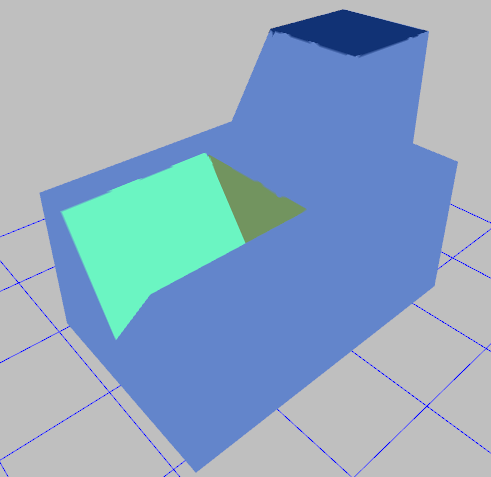
\includegraphics[width=\linewidth]{../resources/watershed/fc028_WS4.2.0.png}
		\caption{Shallow merge with a high merge threshold}
		\label{sfig:ws_4.2.0}
	\end{subfigure}
	\hfill
	\begin{subfigure}{0.45\textwidth}
		\centering
		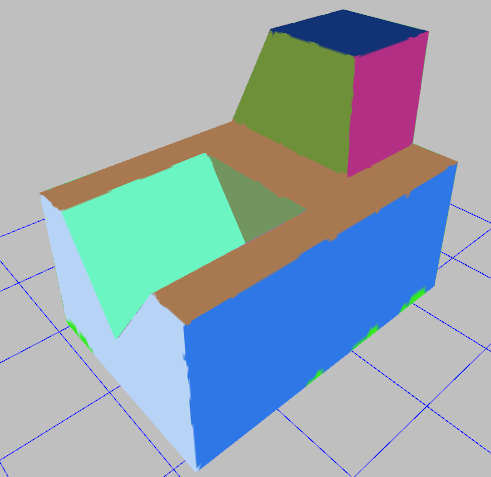
\includegraphics[width=\linewidth]{../resources/watershed/fc028_WS4.2.1.png}
		\caption{\raggedright Shallow merge with a lower merge threshold}
		\label{sfig:ws_4.2.1}
	\end{subfigure}
\caption{
Results from Watershed segmentation step 4.2 with a high merge threshold (a) and a lower merge threshold (b).
}
\end{figure}

Figures \ref{sfig:ws_4.2.0} and \ref{sfig:ws_4.2.1} show the results post \textit{shallow-merge}.
If the merge threshold is too high, useful regions will be merged together into a large composite mesh section, as can be seen in figure \ref{sfig:ws_4.2.0}.
figure \ref{sfig:ws_4.2.1} shows the result of a merge threshold more appropriate for the mesh shown.
Because each model has different geometry and meshing, a certain merge threshold may work well for one model, yet work poorly for another.
A certain merge threshold may not even work well for the entirety of a single model.
This is why the \textit{3D Segmentation} process is iterative.
By starting with a relatively high merge threshold exponent (0.95) and decreasing, all surfaces should eventually be classified as a certain primitive.

\subsubsection{Boundary Smoothing}
This step is more post-processing and ``cleaning'' of the mesh region boundary than actual segmentation.
Due to randomness in the mesh there are situations where a vertex is connected to its region by a single edge.
Such vertices are named ``web1'' points, due to them having a single webbed connection to their region's perimeter.
In order to smooth the region boundary, an attempt is made to find an adjacent mesh region more suitable to possess each web1 point.
Because vertices with only 3 edges are exceedingly rare in well meshed models, it is sufficient to transfer ownership of the web1 point to the adjacent region with the highest number of connecing edges.
Thus, for example, A vertex assigned to region 4 through Minima Descent with edges connecting to regions 4, 10, 12, and 12, would be transferred to region 12.
No explicit tie breaking mechanism was deemed necessary, but lower numbered regions are likely given priority due to how the code was written.
% At one point perimeter vertices with 3 or more connections to other same-region perimeter vertices were considered a problem,...

% TODO: take a pair of screenshots to illustrate WS5:boundary smoothing?

\subsection{Surface Classification}
Mesh regions received from Watershed segmentation need to be classified so that the appropriate UV-map is assigned to them.
The primitives against which each mesh region is tested are: planes, cylinders, and ellipsoids.
Because Watershed segments along regions of high curvature, perimeter vertices were excluded from the tests described below.
The main idea was to perform some tests on a the mesh region's vertices to obtain an educated guess as to the surface's class, and confirm or reject the guess by attempting to fit the assumed shape to the surface and examining the resultant error value.
This works well for planar classification because measuring the distance of a given point from the regression plane is trivial.
Computing the distance from a given point to an ellipse or other conic shape is non-trivial and, at the time of writing, no exact algebraic solution was found.
In place of an exact distance function, the sum of squared residuals was used.
For example, a point on a conic section should satisfy equation \ref{eq:gen_conic}, but for a point \textit{almost} on a conic section, the result will be non-zero:
\begin{equation}
	R(x,y) = Ax^2 + Bxy + Cy^2 + Dx + Ey + F,
\end{equation}
where $R(x,y)$ is the residual. The error function then becomes:
\begin{equation}
	e = \sum_i \left(Ax_i^2 + Bx_i y_i + Cy_i^2 + Dx_i + Ey_i + F\right)^2
\end{equation}
While easy to calculate, this value is unreliable as an indicator of whether or not the given surface is actually a conic surface.
Through testing cases were in which obviously non-cylindric surfaces yielded extremely low error values.
Due to this realization greater emphasis was placed on the initial classification step.

\subsubsection{Planar Classification}
Various tests were devised to determine if a given mesh region can be classified as planar.
An early idea was to cluster the normals of the given mesh region, and perform a sort of statistical analysis on them.
By clustering all normals within a set allowable deviation, the spread in the number of vertices in each cluster should provide insight into the surface type.
One would expect a plane to have a normal-cluster with an overwehelming number of vertices relative to other normal-clusters produced.
By comparison, a cylinder would be expected to have multiple ``significant'' normal-clusters, with similar vertex counts.
This idea was later deemed unnecessarily complex and too susceptible to mesh deviations, and retired in favor of other ideas.

Another idea was to calculate an overall normal vector by performing Principal Component Analysis (PCA) on the vertices' normals.
The vertice's normals were then compared to this overall normal via their dot product.
If too many vertex normals deviated beyond a set angular threshold, the mesh region was determined to be non-planar.
This test works well for ``perfect'' models, such as those from CAD, but is less useful when dealing with noisy meshes and can yield false negatives.

Later, a test that compared the vertices' mean principal curvatures against set thresholds was developed.
Theoretically, the vertices in a planar mesh would exhibit 0 curvature.
Thus, the vertices' 1st principal curvature could be compared against a near-zero threshold, with those above the threshold rejected as non-planar.
Again, this works well for ``clean'' geometry, but not for noisy meshes, because even small deviations in the mesh can inflate the mean curvature.
It \textit{is} possible to set useful curvature thresholds for noisy meshes, but they will be significantly higher than those set for clean meshes, meaning the test does not generalize between clean and unclean meshes.

The second planar test was deemed the most reliable and is used in the submitted algorithm.
As a check on the test, planar regression via Singular Value Decomposition is performed on the mesh region's vertices, and the root mean squared error is reported.
If the RMSE is within a set threshold, the region passes the second check and is classified as planar.

NOTE: perhaps talk about other (untested) ideas?

\subsubsection{Cylindric Classification}
``Cylinder'' (and cylindric) in this context means a surface whose cross section is a conic shape, and has a single axis.
% The single axis criterion was central to later tests conceived during development.

As mentioned in the planar classification section, an early idea was to perform statistical analysis on clustered normals.
An issue with using that method for cylindric classification is that a sphere and a cylinder would yield similar normal-cluster histograms.
(I could probably go into greater detail about why this was a foolish notion, but i would rather write about ideas that had a higher chance of success.)

A test that examined the mean principal curvature values of the mesh region was also considered, but it failed to prove useful for the same reasons outlined in Planar Classification(ref?).
Theoretically, the first principal curvature on the surface of a cylinder would fulfill $|\kappa_1| >> 0$ and the second principal curvature would be approximately 0.
Setting reliable thresholds proved overly difficult.

Another test sought to make use of the vertices' normals by determining the axis direction via PCA, and checking that the dot product between each vertex's normal and the axis was roughly 0:
\begin{equation}
	\vec{v}_{axis} \cdot \vec{n_i} \approx 0.
\end{equation}
This approach has 2 glaring flaws: planes pass this test, and cones do not pass.
% Various tests that take into account the vertices' normals were conceived, but all were either abandoned due to inefficacy, or simply unimplemented due to time constraints.

Currently, the test chosen for planar classification doubles as a cylindric identification.
If a mesh region fails that test, it is non-planar, and thus most likely cylindric.

(?) Talk about future ideas?

? talk about other flaws? This was definitely a weak point in my work

\subsubsection{Ellipsoidal Classification}
The third primitive type would have been ellipsoids, but due to their complexity and time constraints no ellipsoidal indentification or classification functions were developed.
Theoretically, the prinicipal curvature values could also be applied here.
An ellipsoid curves in both surface directions, thus both $|\kappa_1|$ and $|\kappa_2|$ should be noticeably greater than 0.

A flaw with the cylindric tests and this principal curvature test is that they are unable to differentiate between the target surface class and a composite shape.

\section{Geometry Simplification}

\begin{figure}[htb]
	\centering
\begin{tikzpicture}[inner sep=0,
	vertex/.style={circle, radius=2pt,fill, inner sep=2pt,outer sep=0pt}]
	% Nodes
	\matrix (table) [
		matrix of nodes,
		nodes in empty cells,
		row sep=8mm, column sep=6mm,
		nodes={anchor=center}
	] {
		\node[text width=24mm] (MRs) {Classified Mesh Sections}; &[7mm]
		\node[FC-Node, text width=20mm, minimum size=15mm] (cEdges) {Create shared edges}; &
		\node[FC-Node, text width=20mm, minimum size=15mm] (exEdges) {Extend shared edges}; &
		\node[FC-Node, text width=20mm, minimum size=15mm] (cSurfaces) {Create simple surfaces}; &
		\node[text width=24mm, align=left] (SSurfaces) {Simplified Surfaces}; \\
		& & & & \\
	};
\node[FC-Node, fit=(table-2-2)(table-2-3),minimum size=7mm, text width=46mm,label={center:Create shared corners}] (cCorners) {};
	% Connections
	\draw[FC-Arrow] (MRs) -- (cEdges)
		node[pos=0.7, vertex] (split) {};
	\draw[FC-Arrow] (split) -- ($(split |- cEdges.north west)+(0,0.3)$) -| (cSurfaces.north)
		node[pos=0.5] (top) {};
	\draw[FC-Arrow] (cEdges.south) -- (cEdges.south |- cCorners.north);
	\draw[FC-Arrow] (cEdges) -- (exEdges);
	\draw[FC-Arrow] (cEdges) -- (exEdges);
	% \draw [FC-Arrow] ($(cEdges.east)+(0,0.4)$) -- ($(cSurfaces.west)+(0,0.4)$);
	\draw[FC-Arrow] (cCorners.north -| exEdges.south) -- (exEdges.south);
	\draw[FC-Arrow] (exEdges) -- (cSurfaces);
	\draw[FC-Arrow] (cSurfaces) -- (SSurfaces);
	% GeoSimp container node
	\node[thick, dashed,draw, rounded corners=8pt,inner sep=7pt, fit=(split)(top)(cCorners)(cSurfaces),label={90:Geometry Simplification}]{};
\end{tikzpicture}
	\caption{Graphic depiction of the 3D segmentation procedure. Simple surfaces require both shared edges and shared corners, hence the connection from each.}
	\label{fig:GeoSimp}
\end{figure}

The purpose of the geometry simplification step is to create a simplified form for each mesh region provided by Segmentation 3D.
Geometry Simplification's output is a set of ``simple surfaces'' created from the provided mesh regions.
A simple surface contains, among other things, a reference to the mesh region from which it was created, a UV-map, and the unwrapped 2D region outline.
Geometry Simplification follows the block diagram shown in figure \ref{fig:GeoSimp}.
First the \verb|SharedEdges|, edges between mesh regions, are ascertained.
These are used to determine the region corners (``shared corners''), which are then used to finish preparing the shared edges (Extend shared edges).
Finally, the completed shared edges plus the mesh regions are used to create the \verb|simple surfaces|, which are passed on to the next high-level step.

\subsection{Create Shared Edges}
The boundary between two mesh regions is termed a ``shared edge'', because its information is shared between the two mesh regions it divides.
Each shared edge is made up of a list of line segments that approximate the boundary between two mesh regions.
The algorithm to obtain the shared edges is shown split into algorithms \ref{alg:shared_edges_1} and \ref{alg:shared_edges_2}.
The function \textbf{CreateSharedEdges()} can be broken into \textbf{edge discovery} and \textbf{edge refinement}.
% Line 2 sets up list $E_{points}$, in which each entry $i$ is the list of all points for the $i-th$ discovered edge.
% $E_{points}$ is filled throughout \textbf{edge discovery} and in \textbf{edge refinement}
In \textbf{edge discovery} the list of vertices found along each edge is appended to list $E_{points}$.
In \textbf{edge refinement} each edge's list of vertices in $E_{points}$ is transformed into a concise shared edge.

\begin{algorithm}[!htb]
	\caption{createSharedEdges() Part 1: Edge discovery}\label{alg:shared_edges_1}
\begin{algorithmic}[1]
\Function{createSharedEdges}{Surfaces $S$, UV-maps $M$}
	\State new list $E_{points}$ \Comment{Each entry is an edge's list of points}
	% "edge discovery" section
	\State new set $P_{remaining} \leftarrow$ all mesh region perimeter points
	\While{$P_{remaining}$ not empty}\label{alg:shared_edges:while_k_remaining}
		\State point $p_{edge} \leftarrow$ first value in $P_{remaining}$
		\State new queue $K_{tips} \leftarrow p_{edge}$ \Comment{For the beginning of each edge}
		\While{$K_{tips}$ not empty}\label{alg:shared_edges:while_k_tips}
			\State $e_{start} \leftarrow K_{tips}$.dequeue()
			\State \textbf{skip if} $e_{start}$ already in $E_{points}$
			\State new list $P_{edge}$ \Comment{List of points in the current edge}
			\State new queue $P_{search}$ \Comment{Queue of points to search along current edge}
			\While{$P_{search}$ not empty}
				\State $p_{edge} \leftarrow P_{search}$.dequeue()
				\State \textbf{skip if} $p_{edge}$ already in $P_{edge}$
				\State $P_{edge}$.append($p_{edge}$)
				\For{$p_{adj}$ in $p_{edge}$.adjacent\_points}
					\If{$p_{adj}$ on current region boundary}
						\State $P_{search}$.enqueue($p_{adj}$)
					\EndIf
					\If{$p_{adj}$ adjacent to 3+ regions}
						\State $K_{tips}$.enqueue(EdgeStart from $p_{adj}$)
					\EndIf
				\EndFor
			\EndWhile
			\State Remove $P_{edge}$ points from $P_{remaining}$
			\State $E_{points}$.append($P_{edge}$)
		\EndWhile
	\EndWhile
	\algstore{create_shared_edges}
\end{algorithmic}
\end{algorithm}

The \textbf{edge discovery} section, spanning lines 3-28, consists of traversing each mesh section boundary to collect all vertices relevant to that edge and storing them in a list in $E_{points}$.
The outermost \verb|while| loop, beginning on line \ref{alg:shared_edges:while_k_remaining}, ensures that all perimeter points, of all mesh regions, are accounted for.
Each cycle of this loop completely processes a single edge graph.
Edge graph in this context means the collection of edges that are linked to one another.
For example, a cube has a single edge graph, whereas a cylinder has 2 edge graphs, each containing a single edge.
The queue $K_{tips}$ stores potential edge starts.
The next \verb|while| loop, on line \ref{alg:shared_edges:while_k_tips}, processes each potential edge start in $K_{tips}$.
Because multiple edge starts could describe the same edge, it is necessary to check if the current edge start $e_{start}$ is already contained in an edge in $E_{points}$ (line 9).
The queue $P_{search}$ created on line 11 handles the points found to be on the current edge.
The subsequent \verb|while| loop processes $P_{search}$ until empty, first checking for duplicates, appending the current edge point $p_{edge}$ to the list of current edge points $P_{edge}$, and finally checking its neighbors for new edge points.
A vertex is deemed to be on the edge between regions $A$ and $B$ if it is either in $A$ and adjacent to $B$ or in $B$ and adjacent to $A$.
Lines 20-22 show that if a vertex adjacent to 3 or more regions is found, an edge start is created from it and enqueued to $K_{tips}$.
After $P_{search}$ is exhausted, $P_{edge}$ is assumed to contain all points on the current edge.
These points are then removed from the overall point set $P_{remaining}$ and appended to $E_{points}$, concluding the $K_{tips}$ \verb|while| loop.

\begin{algorithm}[htb]
	\caption{CreateSharedEdges() Part 2: Edge refinement}\label{alg:shared_edges_2}
\begin{algorithmic}[1]
	\algrestore{create_shared_edges}
	% "edge refinement" section
	% \State comment about source of muv1/2
	\State new list $E$ \Comment{List of shared edges}
	\For{$P_{edge}$ in $E_{points}$}\label{alg:edge_refinement_for}
		\State Determine the surfaces $s_1$ and $s_2$ adjacent current point line $P_{edge}$
		\State Obtain UV-maps $m_{UV1}$ and $m_{UV1}$ from $s_1$, $s_2$ and $M$
		\State ClampPointsToSurfaces($P_{edge}$, $m_{UV1}$, $m_{UV2}$)\label{alg:edge_refinement_clamp_pts}
		\State SortEdgePoints($P_{edge}$)
		\State $E$.append(SharedEdge($P_{edge}$))
	\EndFor
	\State \textbf{return} $E$
\EndFunction
\end{algorithmic}
\end{algorithm}

\textbf{Edge refinement} is, relative to \textbf{edge discovery}, fairly simple.
A new list $E$ is created to store the final shared edges.
The \verb|for| loop on line \ref{alg:edge_refinement_for} iterates through the lists of edge vertices in $E_{points}$, attempting to create a shared edge from each.
On line \ref{alg:edge_refinement_clamp_pts} \verb|ClampPointsToSurfaces()| forces the edge points onto an idealized representation of the two bordering mesh sections.
For an edge between two planar surfaces, this would force all points to be colinear.
Next the clamped points are sorted according to position along the line using \verb|SortEdgePoints()|.
Finally a shared edge is created from the edge points, and then appended to $E$.
Within the creation of a shared edge the RDP algorithm is used to simplify the line down to only the critical points.
% The complete list of vertices is simplified via the Ramer-Douglas-Peucker (RDP) algorithm\cite{RDP_line_reduction}.
The mesh's mean edge length is used as the tolerance width in the RDP algorithm.
Once all point lists in $E_{points}$ have been processed, the list $E$ is returned, and \verb|CreateSharedEdges()| is complete.

\subsection{Create Shared Corners}

\begin{algorithm}[!b]
	\caption{Create shared corners}\label{alg:shared_corners}
\begin{algorithmic}[1]
\Function{createSharedCorners}{Region edges list $E_{R,E}$}
	\State new list $C$ \Comment{To store the shared corners}
	\For{$E_r$ in $E_{R,E}$}
		\State new list $T$ \Comment{Set of all line tips relevant to a given region}
		\For{edge $e$ in $E_r$}
			\State $T$.append($e$.start)
			\State $T$.append($e$.end)
		\EndFor
		\While{$T$ not empty}
			\State new line tip $t_{target} \leftarrow$ first in $T$
			\State $T$.erase($t_{target}$)
			\State new line tip $t_{near} \leftarrow T$.closestTo($t_{target}$)
			% \State new line tip $t_{near} \leftarrow$ first in $T$
			% \State new point $p_{target} \leftarrow l_{target}$.position
			% \State new float $d \leftarrow \infty$
			% \For{$t$ in $T$} \Comment{Find the line tip closest to $t_{target}$}
			% 	\State new point $p \leftarrow t$.position
			% 	\If{distance($p_{target}$, $p$) < $d$}
			% 		\State $d \leftarrow$ distance($p_{target}$, $p$)
			% 		\State $t_{near} \leftarrow t$
			% 	\EndIf
			% \EndFor
			% check existing shared corners if any contain near/target l
			\State new boolean $b_{found} \leftarrow$ false
			\For{$c$ in $C$}
				\If{$c$.contains($t_{target}$) or $c$.contains($t_{near}$)}
					\State $c$.insert($t_{target}$)
					\State $c$.insert($t_{near}$)
					\State $b_{found} \leftarrow$ true
					\State \textbf{break}
				\EndIf
			\EndFor
			\If{not $b_{found}$}
				\State new shared corner $c$($t_{target}$, $t_{near}$)
				\State $C$.append($c$)
			\EndIf
			\State $T$.erase($t_{near}$)
		\EndWhile
	\EndFor
	\State \textbf{return} $C$
\EndFunction
\end{algorithmic}
\end{algorithm}

Shared corners are used to simplify the process of extending the shared edges to the regions they abut.
The process of creating shared corners $C$ is outlined in algorithm \ref{alg:shared_corners}.
The \verb|CreateSharedCorners()| argument $E_{R,E}$ is a list, where each entry is the list of edges that border the mesh region indexed by the $E_{R,E}$ index.
That is, the $i$-th item in $E_{R,E}$ is the list of edges that border mesh region $i$.
Determining which line tips match is facilitated by each item in $E_{R,E}$ only containing the edges relevant to a given mesh region.
% Having a list of the edges relevant to a single mesh region facilitates determining which line tips match.

% \verb|CreateSharedCorners()| is primarily a \verb|for| loop loop
Each iteration of the main \verb|for| loop attempts to create corners from that region's edges.
% The \verb|for| loop starting on line 3 iterates through each list of edges $E_r$ in $E_{R,E}$.
Lines 4-8 create the set $T$ of line tips and initialize it with both line tips from each edge in $E_r$.
The \verb|while| loop starts by finding a pair of matching line tips (lines 10-12).
% Lines 10-12 pull the first line tip from $T$ and find the closest line tip to the removed one.
% The remainder of the while loop serves to check if any existing shared corner $c$ in $C$ already contain either of the matching line tips $t_{target}$ or $t_{near}$.
Next an existing shared corner $c$ that already contains either matching line tip is sought.
If such a shared corner is found $t_{target}$ and $t_{near}$ are added to it.
Otherwise a new shared corner is created from the matching line tips and appended to $C$.
Finally, the list of shared corners $C$ is returned.

\subsection{Extend Shared Edges}
% Another meaningful name for this would be "force line tip coincidence", at least for the fn
At this point the shared edges align with the regions they divide, but likely do not extend to meet the shared corners or each other.
\verb|ClampLineTips()|, described in algorithm \ref{alg:clamp_line_tips}, exists to rectify this.

\begin{algorithm}[hb]
\caption{Clamp Line Tips}\label{alg:clamp_line_tips}
\begin{algorithmic}[1]
\Function{clampLineTips}{$C$, $S$, $M_{UV}$}
	\For{$c$ in $C$}
		\State new set $S_{corner} \leftarrow c$.adjoiningSurfaces() \Comment{The set of surfaces that adjoin $c$}
		\For{line tip $t$ in $c$.lineTips()}
			\State new set $S_{edge} \leftarrow E$[$t$].adjacentRegions()
			\State new set $S_{diff} \leftarrow S_{corner} - S_{edge}$ \Comment{The set difference of $S_{corner}$ and $S_{edge}$}
			% \State new uint $i_{UV} \leftarrow S$[$S_{diff}$.first].UVMapIndex
			\State Obtain new UV-map $m_{UV}$ representing $S_{diff}$ from $M_{UV}$
			% \State new UV-map $m_{UV} \leftarrow M_{UV}$[$i_{UV}$]
			% \State $E$[$t$.edgeIndex].clampTipPoint($m_{UV}$, $t$.tipType)\label{alg:clamp_tip_point}
			\State $t$.clampTipPoint($m_{UV}$)\label{alg:clamp_tip_point}
		\EndFor
	\EndFor
\EndFunction
\end{algorithmic}
\end{algorithm}

The \verb|ClampLineTips| arguments are as follows:
% $E$: the shared edges,
$C$: the shared corners, $S$: the mesh surfaces, and $M_{UV}$: the list of UV-maps.
% The objective is to find for a given line tip the region, and its corresponding UV-map, that set the line tip's position along the line tip direction.
The objective is to find the surface that a given line tip points to, and use that surface's UV-map to force the line tip onto said surface.
The inner \verb|for| loop iterates through the line tips of the current shared corner.
To determine to which surface a line tip points, the set $S_{edge}$ of surfaces adjacent to the line tip $t$ is subtracted from the set $S_{corner}$ of surfaces adjacent to the current shared corner $c$.
% For a typical 3-surface corner, the set difference $S_{diff}$ will contain a single element,
The number of elements in the set difference $S_{diff}$ is dependent on the number surfaces joined by the current shared corner.
Although $S_{diff}$ can contain more than one element, it matters not which is chosen as the extension target for the line tip.
Next the UV-map belonging to the surface in $S_{diff}$ is obtained.
On line \ref{alg:clamp_tip_point} the line tip $t$ is forced to lie at the intersection of its tangent and the extension target surface.
Figure \ref{fig:extend_shared_edges} below shows the before and after of applying \verb|ClampLineTips| to a set of shared edges.

\begin{figure}[htb]
	\centering
	\begin{subfigure}{0.45\textwidth}
		\centering
		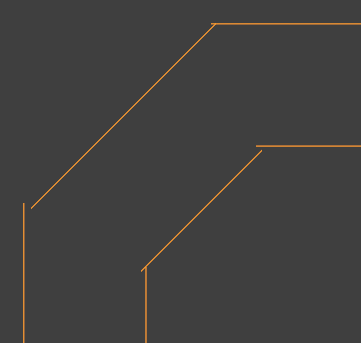
\includegraphics[width=\linewidth]{../resources/geo_simp/1505020_shared_edges.png}
		\caption{Shared edges post \textit{create shared edges}}
		\label{sfig:gs_shared_edges}
	\end{subfigure}
	\hfill
	\begin{subfigure}{0.45\textwidth}
		\centering
		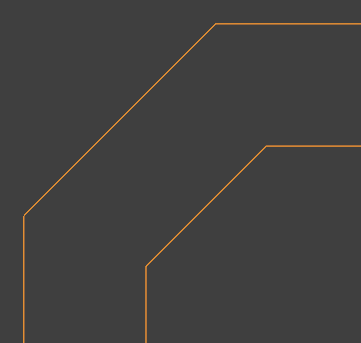
\includegraphics[width=\linewidth]{../resources/geo_simp/1505020_shared_edges_clamped.png}
		\caption{Shared edges post \textit{extend shared edges}}
		\label{sfig:gs_shared_edges_clamped}
	\end{subfigure}
\caption{
The shared edges from test object ``1505020'' Before and after \textit{extend shared edges}
}
	\label{fig:extend_shared_edges}
\end{figure}

As can be seen in figure \ref{sfig:gs_shared_edges} ``unclamped'' shared edges are decent, but noticeably unconnected.
Figure \ref{sfig:gs_shared_edges_clamped} shows the same edges post \textit{extend shared edges} and noticeably connected.

\subsection{Create Simple Surfaces}
A simple surface is created from a mesh region and the shared edges that border said mesh region.
% How are simple surfaces formed?
The bulk of the procedure to create a simple surface is the process to form the surface's outlines from the given shared edges.
This process is described in detail in algorithm \ref{alg:find_outlines}.
% Given a mesh region and the previously created shared edges as input, the simple surface first collects the edges and corners that border the source mesh region.
% Next the outlines of the mesh region are generated from the shared edges (see below...)

% find_outlines(shared_corners, corner_indices, edge_indices, uv_map_index, uv_mappings);
\begin{algorithm}[!htb]
	\caption{Find outlines}\label{alg:find_outlines}
\begin{algorithmic}[1]
\Function{findOutlines}{Shared edges $E_{shared}$, Line tips $T$, UV-map $m$}
	\State new set O \Comment{To store the created outlines}
	\State new list $T_{sorted} \leftarrow T$ \Comment{Local copy of $T$ to be sorted throughout function}
	% \State new uint $vii \leftarrow 0$
	\State new set $E$ from each edge associated with $T$

	\While{$E$ not empty}
		\State new list $T_{outline}$ \Comment{For the outline's line tips}
		\State new edge $e_0 \leftarrow E$.first
		% \State new line tip $t_{target} \leftarrow$ LineTip{$e_0$, END}
		\State new line tip $t_{target}$ derived from END of $e_0$
		\Repeat
			\State $t_{target} \leftarrow$ findNextLineTip($t_{target}$, $E_{shared}$)
			\State $T_{outline}$.append($t_{target}$)
			\State $E$.erase($t_{target}$.edge)
		\Until{$t_{target}$.edge = $e_0$}
		\State Update $T_{sorted}$ from $T_{outline}$
		\State new list $P_{corner}$
		\For{$t$ in $T_{outline}$}
			\State new list $P$ from $t$'s shared edge's points
			\If{$t$ is a line tip END}
				\State reverse(P)
			\EndIf
			\For{$p$ in $P$}
				\State new $p_{UV} \leftarrow m$.transformToUV($p$)
				\State $P_{corner}$.append($p_{UV}$)
			\EndFor
		\EndFor
		\State $O$.append($P_{corner}$)
	\EndWhile
	\State $T \leftarrow T_{sorted}$
	\State \textbf{return} $O$
\EndFunction
\end{algorithmic}
\end{algorithm}

The purpose of \verb|FindOutlines| is to determine all outlines associated with the simple surface under construction.
An outline in this context is the surface's boundary lines \textit{and} any holes the surface may have.
Line 4 sets up the set of edges associated with line tips $T$.
Each iteration of the function's \verb|while| loop produces a new outline.
On line 8 a line tip $t_{target}$ is created as the end line tip of edge $e_0$.
This serves as the initial line tip ``targeted'', and as the end condition for the \verb|repeat-until| loop.
The function to find the next sequential line tip, \verb|findNextLineTip|, is shown in algorithm \ref{alg:next_line_tip}.
When a new $t_{target}$ is found it is added to the outline and its edge is erased from $E$ to show that it has been accounted for.
When $t_{target}$'s edge equates to $e_0$ the loop and outline are complete.
The remainder of the \verb|while| loop converts the outline as a list of line tips to a list of points.
On line 17 $P$ is the list of points from the shared edge associated with line tip $t$.
For a straight line this is only 2 points, but for a curve there could be a much larger number of points.
The \verb|if| statement on line 18 ensures that the outline's points are properly sequential, by reversing $P$ if the associated line tip is an END line tip.
Once $P$ is complete, each point $p$ therein	is transformed to the surface's local coordinate system and appended to $P_{corner}$.
The completed list of local points is then added to	the list of outlines $O$.
Once all edges in $E$ have been accounted for in an outline, the outlines are returned and the function finished.
% The outlines created are sorted by descending area size, so that the first outline is guaranteed to be the surface's outline and the remaining outlines are holes in the surface.

\begin{algorithm}[htb]
	\caption{Find next line tip}\label{alg:next_line_tip}
\begin{algorithmic}[1]
\Function{findNextLineTip}{Line tip $t_{target}$, edges $E$}
	\State new point $p_{target} \leftarrow$ position of $t_{target}$
	\State new real $d_{nearest} \leftarrow \infty$
	\State new line tip $t_{nearest}$
	\For{$e$ in $E$}
		\For{$t_{type}$ in [START, END]}
			\State new line tip $t_{temp}$ from $e$ and $t_{type}$
			\State new real $d \leftarrow$ distance from $p_{target}$ to $t_{temp}$'s position
			\If{$t_{temp}$ is not $t_{target}$ AND $d$ < $d_{nearest}$}
				\State $d_{nearest} \leftarrow d$
				\State $t_{closest} \leftarrow t_{temp}$
			\EndIf
		\EndFor
	\EndFor
	\If{line tip $t_{nearest}$ is START type}
		\State \textbf{return} line tip from END of $t_{nearest}$.edge
	\Else
		\State \textbf{return} line tip from START of $t_{nearest}$.edge
	\EndIf
\EndFunction
\end{algorithmic}
\end{algorithm}

The purpose of \verb|findNextLineTip| is to find the next sequential line tip given the current one ($t_{target}$) and a list edges.
% To do so, the line tip closest but not equal to $t_{target}$ is sought,...from the given list of edges.
The nested \verb|for| loops iterate both ends of each edge in $E$ to find the line tip closest but not equal to $t_{target}$.
This yields the sequential next edge, but $t_{nearest}$ is not the line tip sought, because it is still approximately coincident to $t_{target}$.
Thus, the line tip sought, is the one \textit{opposite} along the edge of $t_{nearest}$.
Hence the \verb|if-else| statements on lines 15-18.

Once the creation of simple surfaces is complete, they are passed on to the next high-level step: \textit{2D Segmentation}.
(Is there anything else i should say about simple surfaces?)

\section{2D Segmentation}
This is Interior Edge Extension
The idea was that downstream components requried convex shapes to facilitate local path planning.
In hindsight, surfaces need not be completely convex, but merely \textit{mostly} convex.

\section{Surface Path Planning}
This is effectively Boustrophedon

\section{Modified Traveling Salesman Problem}
Normal TSP should have already been described in \ref{background}, so no need to rehash that.
Only need to talk about the modifications and how it would have been applied...

\section{Inverse Kinematics}
Talk about how the InvKin from the robot could be used, but a custom one would (likely) be necessary to incorporate the rotary table

